\chapter{Estado de la cuestión}
\label{cap:estadoDeLaCuestion}

\begin{resumen}
En este capítulo vamos a hablar sobre los videojuegos de rol, introducir un poco su historia, hablar sobre el desarrollo de videojuegos, qué es un motor, para qué sirve, qué lo compone, qué es un editor, para qué sirve, y cuáles son los editores especializados en el desarrollo de videojuegos de rol.
\end{resumen}

\section{Sobre los videojuegos de rol}
Para poder definir qué es un videojuego de rol necesitaremos primero entender \textit{qué es un videojuego} y \textit{qué es un juego de rol}.

\medskip

Definir qué es un videojuego es una tarea bastante complicada, sobre todo teniendo en cuenta los matices con los que podemos definirlo (académicos, de diseño, experimentales o tecnológicos). Una de las definiciones más acertadas nos la da \cite{EspositoVJ}, que lo define como \comillas{un \textit{juego} que se \textit{juega} gracias a un \textit{aparato audiovisual}, y que puede estar basado en una \textit{historia}}. El propio \citeauthor{EspositoVJ} se encarga de definir qué es el \textit{juego}, qué es \textit{jugar}, qué es el \textit{aparato audiovisual} y qué es la \textit{historia}. La diferencia fundamental de los juegos tradicionales frente a los videojuegos es la existencia de ese \textit{aparato audiovisual} (videoconsolas, ordenador, dispositivos móviles) que pueda ofrecer una interacción \comillas{humano-máquina}, ya que es esta interacción recíproca la que hace que los videojuegos sean videojuegos y no otro tipo de entretenimiento multimedia.

\medskip

Los juegos de rol, al haber nacido desde juegos de mesa tradicionales, han tenido el suficiente tiempo como para poder desarrollarse y poder ajustarse a una definición mucho más precisa, aunque, nuevamente, debido a la amplia variedad de juegos que se pueden catalogar como \comillas{de rol}, es posible que hasta la definición más completa no pueda abarcarlos a todos. \citeauthor{LortzRPG} (\citeyear{LortzRPG}, citado en \cite{FineRPG}), define los juegos de rol como \comillas{todos aquellos juegos que permiten a un determinado número de jugadores asumir los roles de personajes imaginarios y operar con cierto grado de libertad en un entorno imaginario}.

\smallskip

Por otra parte, \citeauthor{TychsenRPG} (\citeyear{TychsenRPG}, citado en \citet*{RPGH&D}) enumera los elementos imprescindibles que un juego debe tener para ser considerado como juego de rol:
\begin{itemize}
	\item Narrar una historia adecuándose a una serie de reglas. Tanto la historia como las reglas son únicas para cada juego.
	\item Reglas, múltiples participantes (al menos dos) y un mundo ficticio sobre el que se va a desarrollar la acción. Todos los participantes deben conocer previamente la ambientación, el entorno y las reglas.
	\item La gran mayoría de participantes controlarán, como mínimo, a un personaje durante toda la partida, y será con ese o esos personajes con quienes interactuará con el entorno.
	\item La existencia, por lo general, de un \textit{director de juego} (GM, \textit{gamemaster}), que será el responsable de gestionar aquellos elementos del juego o del entorno ficticio que no se encuentran bajo el control directo de los jugadores.
\end{itemize}

\medskip

Ahora que ya sabemos \textit{qué es un videojuego} y \textit{qué es un juego de rol}, y pese a que no podemos dar una definición válida para todos los videojuegos que estén en esta categoría, definiremos un videojuego de rol (RPG, \textit{role-playing game}, o también, más raramente, CRPG, \textit{computer role-playing game}) como todo aquel programa \textit{software}, con carácter lúdico, que permita a sus usuarios encarnar el rol de uno o varios personajes en un mundo ficticio, donde pueden tomar decisiones, interactuar con su entorno o mundo con cierta libertad y desarrollar una narrativa para conseguir un determinado objetivo.

\smallskip

Como se ha mencionado anteriormente, esta definición vale para la gran mayoría de RPG; pero, si pensamos en los videojuegos que se venden cada día en las tiendas, una proporción significativa de estos puede encajar dentro de la definición anterior sin necesariamente tener que ser un RPG, ya que prácticamente en todos se encarna el rol de un personaje, casi todos permiten una interacción con el entorno y todos tienen un objetivo final. Esto nos lleva a plantearnos si las clasificaciones de videojuegos según su género son demasiado limitadas para los videojuegos actuales.

\subsection{El problema de los géneros de videojuegos}
Antes de adentrarnos en los RPG, veremos por qué las distintas clasificaciones de videojuegos atendiendo a características similares tienen bastantes lagunas a la hora de categorizar las entregas más modernas.

\medskip

Los primeros intentos de clasificar los videojuegos mediante características comunes surgen en la década de los 80, principalmente por diseñadores y desarrolladores, como \cite{Crawford84}, quien los categorizó entre aquellos que \textit{requieren de habilidades previas por parte del usuario} (como juegos de combate o de carreras), y \textit{juegos de estrategia} (que engloba al resto de juegos, como los de aventuras, los educativos, y los RPG). Estas categorías son \textit{funcionales}, se centran en las mecánicas de juego y enfatizan cómo los jugadores interactúan con el sistema.

\smallskip

En la actualidad, los distintos géneros vienen dados por una mezcla de mecánicas, temas, elementos narrativos, estética, lugar de origen y plataforma, y están gravemente influenciados por las tendencias del mercado, discursos mediáticos y la propia percepción de los jugadores. También, muchas veces se quiere categorizar a los videojuegos con etiquetas propias de otras modalidades, como el cine o la literatura, que son incapaces de capturar los aspectos únicos que definen a un videojuego.

\smallskip

\cite{FailGeneros} argumentan que las categorías existentes a día de hoy se quedan cortas para satisfacer los propósitos del género en videojuegos (identidad, agrupación, \textit{marketing} y educación), ya que dada la gran diversidad de juegos que tenemos ahora, resulta casi imposible poder agrupar la naturaleza multifacética de estos en etiquetas tan \comillas{tradicionales}.

\figura{Bitmap/botw}{width=0.7\textwidth}{fig:botw}{Escena de juego de \cite{BOTW}, extraída de \cite{BOTWForbes}.}

\smallskip

Pongamos el ejemplo de uno de los juegos más exitosos de la última década, \citegame{The Legend of Zelda: Breath of the Wild}{BOTW}, que mezcla elementos de libre exploración (lo que lo convertiría en un \textit{sandbox} o \comillas{juego libre}), como bien podemos apreciar en la figura \ref{fig:botw} por el enorme mundo en el que se desarrolla la acción; acción en tiempo real e investigación y resolución de rompecabezas (lo que lo convertiría en un juego de \comillas{acción-aventura}); y la progresión en tiempo real del personaje característica de los RPG (puedes ir consiguiendo nuevas habilidades o mejorando el equipamiento). Es por eso que muchas veces tenemos géneros intermedios, como en este caso, que podríamos considerar a \textit{Breath of the Wild} como un RPG de acción (ARPG, \textit{action role-playing game}, que igualmente siguen sin englobar a la increíble diversidad de juegos. Este problema también se puede aplicar a la inversa, donde juegos como \citegame{Undertale}{Undertale}, esencialmente un RPG, tiene elementos, como el combate, propios de otro género de juegos.

\smallskip

Hay muchas formas de evitar este problema, y quizá la mejor solución sea dejar de considerar a los géneros como \comillas{cajones estancos} en los que un videojuego no pueda pertenecer a dos de estas categorías simultáneamente \citep{Apperley}, sino que sean más bien un espectro, sin fronteras establecidas, en el que un videojuego pueda caer entre dos categorías distintas.

\medskip

En resumen, antes de categorizar un videojuego en según qué género, hay que entender que resulta imposible que este se reduzca a una fórmula fija, sino que hay que entenderlo como una combinación fluida de mecánicas, elementos narrativos, temas y estética, que varían de juego a juego.

\subsection{Historia de los videojuegos de rol}

\figura{Bitmap/dnd1975}{width=0.6\textwidth}{fig:dnd1975}{Interfaz de \cite{dnd}, extraída de \cite{dndimage}.}

Es a mediados de la década de los 70 cuando podemos hablar del nacimiento de los videojuegos de rol. Dadas las limitaciones tecnológicas de la época, los RPG primitivos no eran más que simples adaptaciones de juegos de mesa ya existentes por entonces, como \citegame{dnd}{dnd}, una adaptación de \citegame{Dungeons \& Dragons}{ogdnd}, quizás el juego de rol más famoso, que mezcla mecánicas de combate con temas fantásticos. De \textit{Dungeons \& Dragons} se ha adoptado en la gran mayoría de juegos el lanzar los dados, las estadísticas de los personajes (por ejemplo, inteligencia o fuerza), o sistemas de niveles. 

\smallskip

Estos primeros juegos contaban con interfaces basadas en texto, resaltadas con colores muy vivos, y pocos \textit{sprites}, muchas veces llegando a dibujarlos utilizando caracteres ASCII (ver figura \ref{fig:dnd1975}), y normalmente estaban programados en los grandes ordenadores que se encontraban en campus universitarios como los de Harvard o la Universidad de Illinois. Esta primera etapa, \cite{barton2008dungeons} la denomina como la etapa de \comillas{años oscuros} (en un símil con los años oscuros del Medievo europeo), principalmente por lo anteriormente mencionado, pero también por la escasa información que tenemos hoy en día sobre estos juegos, ya que muchos no se han conservado son \textit{lost media} (aquellos materiales multimedia que ya no existen en ningún formato y para los cuales no hay ninguna copia disponible).

\smallskip

\begin{figure}[t]
\centering
\begin{SubFloat}
{\label{fig:rogue}%
	Captura de \cite{rogue}, extraída de \cite{rogueimg}}%
	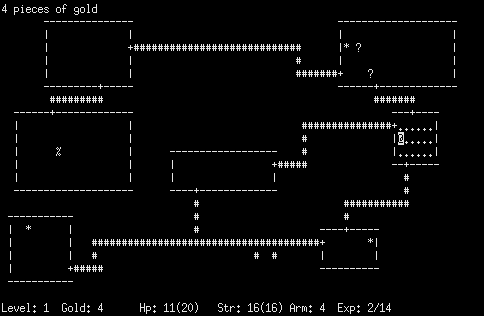
\includegraphics[width=0.45\textwidth]{Imagenes/Bitmap/rogue}%
\end{SubFloat}
\qquad
\begin{SubFloat}
{\label{fig:ultima}%
	Captura de \cite{ultima}, extraída de \cite{ultimaimg}}%
	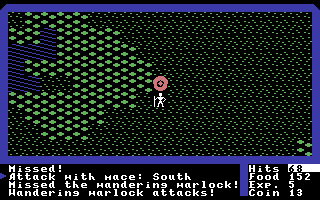
\includegraphics[width=0.45\textwidth]{Imagenes/Bitmap/ultima}%
\end{SubFloat}
\caption{Capturas de \textit{Rogue} y \textit{Ultima}. \label{fig:rogueultima}}
\end{figure}

De esta primera etapa también cabe mencionar tres videojuegos que dieron comienzo a tres distintos subgéneros dentro de los RPG: 
\begin{itemize}
\item \citegame{Rogue}{rogue}, que dio lugar a los videojuegos de mazmorra o \textit{roguelikes}, caracterizados por la generación aleatoria de un laberinto o mazmorra (ver figura \ref{fig:rogue}) en el que se desarrolla una aventura basada por turnos. En este tipo de juegos la muerte es permanente, y al perder la partida se empieza en una nueva desde cero. 
\item \citegame{Wizardry}{wizardry}, que dio lugar a los videojuegos de exploración de mazmorra o \textit{dungeon crawlers}, similares a los anteriores, pero centrados en la exploración de la mazmorra, con un énfasis en la progresión de los personajes y de la gestión de la \textit{party} o escuadrón (el conjunto de personajes que juntos intentan alcanzar objetivos comunes). 
\item \citegame{Ultima}{ultima}, que dio lugar a los RPG de mundo abierto. En esta clase de juegos, los jugadores pueden explorar libremente ciudades, mazmorras, bosques y otro tipo de entornos, manteniendo las mecánicas tradicionales de otros RPG (ver figura \ref{fig:ultima}). 
\end{itemize}

\medskip

Con el salto tecnológico que hubo a mediados de la década de los 80, los RPG comienzan a separase cada vez más de ser meras adaptaciones de juegos ya existentes a desarrollar sus propias historias. A partir de esta época encontramos dos corrientes bastante diferenciadas de RPG, los \comillas{occidentales} (WRPG, \textit{Western role-playing game}), con más libertad de decisión para los jugadores tanto en personalización como en la historia, y con temáticas realistas (como los anteriormente mencionados \textit{Rogue}, \textit{Wizardry} y \textit{Ultima}); y los \comillas{orientales} o \comillas{japoneses} (JRPG, \textit{Japanese role-playing game}, por ser Japón el país que más videojuegos de este tipo produce), centrados en una narrativa lineal con temáticas fantásticas y mecánicas basadas por turnos. Dos grandes videojuegos que definieron el género de los JRPG son \citegame{Dragon Quest}{dq} y \citegame{Final Fantasy}{ff}, cuyas sagas permanecen hasta nuestros días con nuevas entregas cada pocos años. Son estos años de apogeo de los RPG los que \citeauthor{barton2008dungeons} denomina como \comillas{etapa dorada}.

\medskip

La década de los 90 supuso un grave declive para los RPG, especialmente en los mercados occidentales, ya que la aparición de juegos de acción en 3D, como \citegame{Doom}{doom}, \citegame{Quake}{quake} o \citegame{Tomb Raider}{lc}, hizo que el mercado cambiase hacia este tipo de juegos, mucho más rápidos y frenéticos que los RPG, que se consideraban obsoletos, con una pesada carga textual y mucho más lentos de jugar. También, la aparición de videoconsolas mucho más potentes y baratas, como la \textit{PlayStation} (Sony, 1994) o la \textit{Nintendo 64} (Nintendo, 1996), para las cuales los RPG occidentales no tenían portabilidad, y los altos costes de desarrollo y producción que supuso el cambio de cartuchos tradicionales a nuevos formatos como CD-ROM, hicieron que los RPG, especialmente los WRPG, tuviesen este gran declive que solo pudo recuperarse con la entrada del nuevo milenio.

\medskip

En el nuevo milenio, que para \citeauthor{barton2008dungeons} es la \comillas{etapa de platino}, surgen sagas con juegos con gráficos mucho más sofisticados y con narrativas mucho más profundas, como la saga \textit{The Elder Scrolls}, más concretamente, su tercera entrega, \citegame{Morrowind}{tes}; la saga \citegame{Fallout}{fallout}; la saga \citegame{Baldur's Gate}{baldurs}; o la saga \citegame{Diablo}{diablo}, que llevan hasta el límite las propias definiciones del género por las mezclas con otros géneros (llegando a ser juegos \comillas{híbridos}). La potencia del \textit{hardware} va en aumento, lo que permite que haya salto cualitativo, tanto gráfico como en jugabilidad, mientras que la tendencia de los mundos abiertos continúa y se mejora, llegando a ser algunos RPG como \citegame{The Elder Scrolls V: Skyrim}{skyrim} o \citegame{The Witcher 3: Wild Hunt}{witcher} algunos de los juegos más jugados de la historia, e incluso ganando múltiples premios a juego del año.

\section{Sobre el desarrollo de videojuegos}
Para entender cómo las empresas o equipos \textit{indies} desarrollan un videojuego desde cero, es imprescindible saber con exactitud cómo funciona el software internamente, y qué formas tienen los programadores o desarrolladores para comunicarse con las entrañas de este durante el proceso de desarrollo. Es por eso que en este apartado veremos lo que es un \textit{motor} y lo que es un \textit{editor}.

\subsection{Motor de videojuegos}
\cite{gregory2018game} define un motor de videojuegos (\textit{game engine}) como todo aquel \textit{software} extensible que, sin apenas modificaciones, puedan servir de base o cimiento para múltiples videojuegos distintos. Ese \textit{software} al que nos referimos es todo el conjunto de herramientas que hacen que por detrás funcione un juego, como por ejemplo, todas las herramientas que se encarguen del \textit{renderizado} o dibujado en pantalla, bien sea en 2D o en 3D, aquellas que se encarguen de la simulación física y detección de colisiones con el entorno, las que se encarguen del sonido, las del \textit{scripting}, animaciones, inteligencia artificial, etc\ldots A todas estas herramientas también se les denomina \textit{motores} (por ejemplo, \textit{motor de render}, \textit{motor de físicas}\ldots).

\smallskip

Todos estos \comillas{submotores} se suelen conocer como \textit{motores de tecnología}, ya que conforman la infraestructura básica técnica del motor más complejo que las usa, y se usan para abstraer la interacción con el \textit{hardware} o sistema operativo; por lo que un motor de videojuegos también podría describirse como \comillas{una capa de abstracción y herramientas orientadas al desarrollo de videojuegos elaborada sobre motores de tecnología}.

\medskip

Debido a las limitaciones tecnológicas de los años 70 y 80, los primeros juegos se desarrollaban todos desde cero, sin apenas compartir código un juego con otro, ya que cada uno necesitaba una lógica optimizada de una determinada manera que otros no necesitaban o no podían utilizar. Además, los juegos solían ser lanzados para una única plataforma, ya que no había la suficiente cantidad de desarrolladores como para portar un juego a otra plataforma distinta con otra serie de requisitos y limitaciones.

\smallskip

No es hasta finales de la década de los 80 cuando los desarrolladores comienzan a reutilizar código entre juegos y surgen los primeros ejemplos de lo que hoy podríamos llamar \comillas{motor}. Uno de los primeros fue el que Shigeru Miyamoto desarrolló en Nintendo para la \textit{Nintendo Entertainment System} \citep{williams2017history}, que se utilizaría en juegos como \citegame{Excitebike}{excitebike} o \citegame{Super Mario Bros.}{smb}.

\smallskip

A principios de los 90 surgen los primeros \comillas{motores modernos}, de la mano de desarrolladoras como \textit{id Software} y juegos como \textit{Doom} o \textit{Quake}, quienes decidieron reutilizar toda la lógica de \textit{renderizado} y los sistemas de simulación física, ya que cada parte estaba desarrollada de manera independiente. Tal fue el éxito que alcanzaron estos dos juegos que muchas empresas prefirieron pagar a \textit{id Software} por una licencia del núcleo del motor y diseñar sus propios recursos, que desarrollar su propio motor desde cero. Una de estas empresas fue \textit{Valve}, quienes desarrollaron uno de los mejores juegos de la historia, \citegame{Half-Life}{hl}, utilizando el motor \textit{GoldSrc} (que es el antecesor del actual motor de Valve, \textit{Source}), una versión modificada del motor de \textit{id Software}.

\medskip

Con la generalización de internet a principios de los 2000, comenzó el auge de comunidades de \textit{modding} en línea, y muchas desarrolladoras comenzaron a lanzar motores de código abierto acompañados por editores de niveles o herramientas de \textit{scripting} (es decir, código de alto nivel, normalmente no compilado, que solo modifica lógica del juego o eventos sin modificar el núcleo del motor).

\smallskip

A día de hoy, las empresas dedican numerosos recursos a la hora de desarrollar nuevos motores, ya que son la parte fundamental del desarrollo de videojuegos, y cada vez son más sofisticados y requieren de gran conocimiento. Por lo general, la gran mayoría de motores actuales suelen ser multiplataforma, algo de lo que hablaremos más adelante.

\smallskip

Los desarrolladores \textit{indie}, por su parte, tienen la posibilidad de poder desarrollar sus propios motores, cuyo contenido no es equiparable al de empresas que producen juegos \textit{triple A} (aquellos juegos producidos por grandes empresas a los que se suelen destinar un alto presupuesto en desarrollo y publicidad); usar motores propietarios de empresas con licencias gratuitas o de poco coste, como por ejemplo \textit{Unity} o \textit{Unreal Engine}; o motores de código abierto, como \textit{Godot}. Por lo general, estos motores ya vienen equipados con un editor, de lo cual hablaremos también posteriormente.

\subsubsection{Componentes de un motor de videojuegos}

\figuratikzparametros{Representación esquemática de la estructura de un juego y su motor con algunos de los componentes principales}{fig:juegoymotor}{
	enginebox/.style={draw, thick, minimum width=9cm, minimum height=6cm, align=center},
  subbox/.style={draw, thick, minimum width=3.8cm, minimum height=1cm, align=center},
  labelbox/.style={draw, thick, minimum width=3cm, minimum height=1cm, align=center}
}{
	\node[labelbox] (game) {\textbf{Juego}};
	
	\node[enginebox, below=1.5cm of game] (engine) {\textbf{Motor}};
	
	\node[subbox, anchor=north west] at ([xshift=0.5cm, yshift=-0.3cm]engine.north west) (render) {Motor de \textit{render}};
	
	\node[subbox, right=0.5cm of render] (physics) {Motor de físicas};
	
	\node[subbox, below=0.3cm of render] (sound) {Motor de sonido};
	
	\node[subbox, right=0.5cm of sound] (input) {Motor de \textit{input}};
	
	\node[subbox, below=2.1cm of render] (net) {Motor de red};
	
	\node[subbox, right=0.5cm of net] (scripting) {Motor de \textit{scripting}};
	
	\node[subbox, below=0.3cm of net] (anim) {Sistema de animación};
	
	\node[subbox, right=0.5cm of anim] (AI) {Motor de IA};
	
	\draw[->, thick] (game.south) -- node[midway, right] {utiliza} (engine.north);
}

Cada motor de videojuegos es distinto, y cada uno incorpora según qué motores de tecnología dependiendo de las necesidades de los programadores o del juego que se esté programando. Siguiendo el esquema provisto en la figura \ref{fig:juegoymotor}, estos son los componentes principales de un motor de videojuegos tanto de grandes empresas, como motores con licencia gratuita, como aquellos de código abierto:
\begin{itemize}
\item \textit{Motor de render o de dibujado}: se encarga de gestionar todas las tareas relacionadas con los gráficos que se muestran en pantalla. Para ello, dibuja objetos bidimensionales o tridimensionales, representados generalmente mediante \comillas{mallas}, a través de técnicas de informática gráfica, como pueden ser la \textit{rasterización} o el trazado de rayos. También es el encargado de gestionar la cámara, luces, sombras, materiales y texturas, y puede aplicar diversos efectos de posprocesado al fotograma final. Muchas de estas tareas las puede definir el propio programador haciendo uso de un tipo de \textit{script} especial llamado \textit{shader}, que en lugar de ejecutarse en el procesador de nuestro computador se ejecuta en el procesador de las tarjetas gráficas. Estos motores suelen ser una capa de abstracción sobre especificaciones estándar para gráficos como \textit{OpenGL}, \textit{Vulkan}, \textit{DirectX} o \textit{Metal}.
\item \textit{Motor de físicas}: se encarga de simular comportamientos físicos realistas. Entre estos comportamientos físicos encontramos las colisiones de objetos con otros objetos o con el entorno, aplicar la fuerza de gravedad a unos determinados objetos, simular las dinámicas de cuerpos rígidos (es decir, el movimiento de cuerpos interconectados bajo la acción de una fuerza externa, como por ejemplo, cajas que se pueden tirar, deslizar o romper), simular dinámicas de cuerpos blandos (similares a los cuerpos rígidos, pero con la posibilidad de que estos se deformen), y, en algunos casos, simulaciones de fluidos y de materiales textiles. Ya que hacer una simulación física es complicado, se suelen utilizar motores de terceros, como por ejemplo \textit{NVIDIA PhysX}, \textit{Havok}, \textit{Bullet} o \textit{Box2D}.
\item \textit{Motor de sonido}: se encarga de gestionar los efectos de sonido, la música, el audio espacial o posicional en dos o tres dimensiones, y todos los efectos sonoros que se pueden aplicar al sonido (reverberación, eco, tono, barrido, mezclado de pistas, oclusión sonora, efecto Doppler, etc\ldots). Algunas librerías utilizadas son \textit{FMOD}, \textit{OpenAL}, \textit{Wwise} o \textit{irrKlang}.
\item \textit{Motor de input o de gestión de la entrada}: se encarga de capturar y procesar eventos de entrada (\textit{input}) del usuario a través de los diversos dispositivos para los que se programe (teclado y ratón, mandos o controladores y pantallas táctiles) y asociarlos a las acciones definidas en el juego.
\item \textit{Sistema de animación}: gestiona animaciones de \textit{sprites} (los elementos gráficos bidimensionales básicos que representan visualmente objetos dentro del juego) o de esqueletos (\textit{rigging}, usados para personajes tridimensionales). Suelen tener soporte para árboles de mezcla y cinemática inversa.
\item \textit{Motor de scripting}: permite escribir lógica específica del juego utilizando lenguajes de programación de alto nivel (como por ejemplo JavaScript, Lua, C\# o Python), separando la implementación del \textit{gameplay} (\comillas{jugabilidad}) del motor. El \textit{scripting} se suele hacer mediante lenguajes de programación interpretados y no compilados, por lo que los cambios más pequeños no requieren de volver a iterar por todo el proceso de compilado del motor o del juego.
\item \textit{Motor de red}: se encarga de gestionar el soporte multijugador, es decir, la comunicación y sincronización cliente-servidor o cliente-cliente. El motor de red también incluye sistemas de emparejamiento (\textit{matchmaking}) y de predicción o interpolación del juego para una simulación fluida en los juegos multijugador.
\item \textit{Motor de inteligencia artificial}: ofrece herramientas para poder crear comportamientos inteligentes artificiales, como por ejemplo, algoritmos de búsqueda de caminos (\textit{pathfinding}, como los algoritmos \textit{A*} o el de Dijkstra), árboles de comportamiento y máquinas de estado, o sistemas de toma de decisiones. Este motor suele tener una conexión directa con el motor de \textit{scripting} para poder definir comportamientos mucho más fácilmente.
\item \textit{Gestor de recursos}: maneja la carga y descarga de recursos como texturas, mallas, sonidos o animaciones, muchas veces bajo demanda del juego mediante gestores de memoria, compresión y de transmisión de datos altamente optimizados.
\item \textit{Sistema de interfaz de usuario}: se encarga de gestionar la barra de estado (HUD, \textit{head-up display}), los menús, texto, botones y otros elementos de la interfaz con los que el usuario pueda interactuar.
\end{itemize}

\subsubsection{Separación entre motor y \textit{gameplay}}
Para poder reusar nuestro motor en múltiples juegos con el menor número de cambios, es necesario saber \textit{cómo y para qué vamos a desarrollar nuestro motor}, y de acuerdo a la decisión que hayamos tomado, establecer la barrera de separación entre el motor y la jugabilidad o \textit{gameplay} del juego.

\medskip

Definimos jugabilidad o \textit{gameplay} como la experiencia interactiva del jugador dentro de un videojuego. Ni \cite{tekinbas2003rules} ni \cite{schell2019art} dan una definición concreta, pero hablan de cómo la interacción entre el jugador, el sistema de reglas del juego y las mecánicas dan lugar a la jugabilidad. No solo cada juego tiene una jugabilidad distinta que depende de las mecánicas y de las reglas que este tenga, sino que puede haber una mecánica emergente que surge a través de las decisiones de cada jugador.

\smallskip

\begin{figure}[t]
\centering
\begin{SubFloat}
	{\label{fig:separaciongeneral}%
		Separación en motores generalistas.}%
		\begin{tikzpicture}
		\draw (0,0) rectangle (3,6);
		\draw (0,2) -- (3, 2);
		\node at (1.5,4) {\textit{Gameplay}};
		\node at (1.5,1) {Motor};
		\end{tikzpicture}
\end{SubFloat}
\qquad
\begin{SubFloat}
	{\label{fig:separacionespecificos}%
		Separación en motores específicos.}%
		\begin{tikzpicture}
		\draw (0,0) rectangle (3,6);
		\draw (0,4) -- (3,4);
		\node at (1.5, 5) {\textit{Gameplay}};
		\node at (1.5, 2) {Motor};
		\end{tikzpicture}
\end{SubFloat}
\caption{Ejemplos de separaciones entre motor y \textit{gameplay} en los distintos motores. \label{fig:separacionesmotgp}}
\end{figure}

Los motores más generalistas que encontramos, como los anteriormente mencionados \textit{Unity}, \textit{Unreal Engine} o \textit{Godot}, debido a que están pensados para poder desarrollar todo tipo de juegos, tienen una barrera de separación entre el motor y el \textit{gameplay} suele estar a la mitad o incluso hacia abajo (ver figura \ref{fig:separaciongeneral}), es decir, que la implementación del juego final que tiene el motor es mínima (el motor es puramente un conjunto de motores de tecnología) y es el desarrollador el que se tiene que encargar de ello. Esta es la gran ventaja que tienen los motores generalistas frente a los específicos, la libertad que dejan al desarrollador para poder implementar la jugabilidad a su manera, con las reglas y mecánicas que él mismo establezca.

\medskip

Si, como es el caso de este proyecto, nos interesa hacer un motor que fije gran parte de la jugabilidad de los juegos que se puedan hacer con él, y que lo único modificable sea la parte artística y visual, tendremos que introducir elementos propios del juego en nuestro motor, dejando menos libertad en el \textit{gameplay} (ver figura \ref{fig:separacionespecificos}). Por ejemplo, nuestro motor dará a los desarrolladores herramientas para poder personalizar los escenarios de combate típicos en juegos RPG, así como un creador de mapas basado en baldosas o \textit{tiles}. 

\smallskip

Este tipo de motores son mucho más rígidos a la hora de poder implementar nuevas funcionalidades y limitan bastante los juegos que se pueden crear con ellos, pero simplifican bastante el desarrollo, y son especialmente útiles para nuevos programadores, que muchas veces se ven abrumados ante tal cantidad de opciones que ofrecen el resto de motores más flexibles, si bien es cierto que no ofrecen la libertad de estos, y la jugabilidad está fijada por el desarrollador del motor y no el del juego.

\subsubsection{Programación dirigida por datos (DDP) en videojuegos}
La programación dirigida por datos (DDP, \textit{data-driven programming}) es un paradigma de diseño en el que gran parte del comportamiento y lógica de un programa están controlados por datos externos en lugar de estar programados en el código fuente de este. Gracias a este paradigma, según \citeauthor{gregory2018game}, ampliamente extendido entre las empresas desarrolladoras de juegos \textit{triple A}, permite a los desarrolladores modificar o expandir el comportamiento del juego sin la necesidad de alterar el motor o el código base de este.

\medskip

Los motores de videojuegos suelen estar programados utilizando lenguajes de  nivel medio (como C o C++, que en la base son lenguajes de alto nivel pero poseen estructuras de acceso a \textit{hardware} como los lenguajes de bajo nivel), ya que se espera tener una gran optimización en estos así como una portabilidad multiplataforma. De todo el gran abanico de lenguajes de nivel medio, un gran porcentaje son lenguajes compilados, es decir, requieren de un \comillas{traductor} (compilador) para generar el código máquina antes de poder ejecutar el programa. Esta compilación depende del tamaño del proyecto y del número de ficheros a compilar, y, en el caso de muchos motores, la compilación puede llegar a tardar decenas de minutos.

\smallskip

Para evitar tener que esperar estos minutos recompilando todo un juego en caso de cambiar un simple parámetro referente al \textit{gameplay}, se opta por la solución más flexible, que es desarrollar todo el juego utilizando datos, generalmente en lenguajes de \textit{scripting}, de alto nivel, como Lua, que no necesitan ser compilados, sino interpretados (la \comillas{traducción} a lenguaje máquina se realiza en ejecución del programa y a medida que sea necesaria) por el motor del juego.

\medskip

Además de reducir los tiempos de compilación en los juegos, lo cual ayuda a reducir los tiempos en las iteraciones de desarrollo, la programación dirigida por datos permite a los diseñadores del juego, que no tienen que ser necesariamente programadores, modificar comportamientos, ajustar parámetros o añadir contenido utilizando archivos de configuración o mediante herramientas visuales.

\medskip

Este paradigma refuerza la ya mencionada separación entre motor y \textit{gameplay}, ya que un mismo motor puede ejecutar distintos juegos (es decir, distintos datos) sin la necesidad de tener que ser recompilado, siempre y cuando los datos estén en un formato y estructura que el motor sea capaz de interpretar.

\medskip

Sin embargo, uno de los principales problemas que supone este paradigma es la depuración del código. Como los datos se suelen almacenar en lenguajes de \textit{scripting}, o en lenguajes de almacenamiento de datos (como JSON o XML), depurar un código o simplemente datos que nuestro motor interpretan, resulta extremadamente difícil si el motor no cuenta con herramientas de depuración integradas específicas para interpretar esos datos.

\subsubsection{Programación multiplataforma}
La programación multiplataforma es una práctica esencial en el desarrollo de videojuegos modernos. Esta característica permite que un mismo juego funcione idénticamente en distintos dispositivos y sistemas operativos (por ejemplo, en el caso de los videojuegos, que funcione en ordenadores Windows, Linux o Mac; en consolas, como PlayStation, Xbox o Nintendo Switch; o en dispositivos móviles, como Android o iOS). Pese a que aumenta las labores de desarrollo del motor (ya que en muchos casos hay que desarrollar módulos específicos para cada una de las plataformas, principalmente de \textit{renderizado}), reduce los costes de mantener un juego y maximiza el alcance de este.

\medskip

Para lograr que un motor sea multiplataforma, hay que tener en cuenta para qué plataformas se va a desarrollar y qué diferencias hay entre cada una de ellas. Es por ello que se suelen utilizar capas de abstracción, que permiten que el núcleo del motor permanezca intacto entre las distintas implementaciones, mientras que son aquellos módulos que difieren de un sistema a otro los que se modifican.

\smallskip

Otro factor a tener en cuenta es la compilación cruzada, es decir, el proceso por el cual el código se compila en una plataforma (principalmente un ordenador con Windows o Linux), pero el ejecutable se genera para una plataforma distinta (por ejemplo, para Android o para PlayStation). Para ello, se deben disponer de herramientas, como CMake, que faciliten la configuración de estas compilaciones.

\medskip

Los principales desafíos en la programación multiplataforma de videojuegos son debidos a las diferencias entre las distintas API (\textit{application programming interface}, interfaz de programación de aplicaciones, es decir, todo el código que permite a dos aplicaciones comunicarse entre sí) de las videoconsolas, tanto en el \textit{render}, como en el manejo de archivos; o las compatibilidades que una librería pueda tener en un sistema o en otro.

\medskip

Otra dificultad añadida es la de la obtención de las distintas SDK (\textit{software development kit}, kit de desarrollo de \textit{software}) y licencias de cada empresa, ya que no son código libre (todo el código está bajo acuerdos de confidencialidad), y muchas de ellas no suelen ser flexibles a la hora de entregar estas licencias a nuevas empresas.

\medskip

Es por ello que muchas veces, en proyectos no profesionales, se suelen utilizar librerías multiplataforma, como SDL, que simplifican bastante la conversión de un sistema a otro y agilizan el desarrollo de un motor; o, directamente, se usan motores multiplataforma, como los ya mencionados \textit{Unity}, \textit{Unreal Engine} o \textit{Godot}.

\subsection{Editor de videojuegos}

\subsubsection{Editores específicos para desarrollo de RPG}

